\documentclass[ignorenonframetext,]{beamer}
\setbeamertemplate{caption}[numbered]
\setbeamertemplate{caption label separator}{: }
\setbeamercolor{caption name}{fg=normal text.fg}
\beamertemplatenavigationsymbolsempty
\usepackage{lmodern}
\usepackage{amssymb,amsmath}
\usepackage{ifxetex,ifluatex}
\usepackage{fixltx2e} % provides \textsubscript
\ifnum 0\ifxetex 1\fi\ifluatex 1\fi=0 % if pdftex
  \usepackage[T1]{fontenc}
  \usepackage[utf8]{inputenc}
\else % if luatex or xelatex
  \ifxetex
    \usepackage{mathspec}
  \else
    \usepackage{fontspec}
  \fi
  \defaultfontfeatures{Ligatures=TeX,Scale=MatchLowercase}
\fi
\usetheme[]{AnnArbor}
\usecolortheme{dolphin}
\usefonttheme{structuresmallcapsserif}
% use upquote if available, for straight quotes in verbatim environments
\IfFileExists{upquote.sty}{\usepackage{upquote}}{}
% use microtype if available
\IfFileExists{microtype.sty}{%
\usepackage{microtype}
\UseMicrotypeSet[protrusion]{basicmath} % disable protrusion for tt fonts
}{}
\newif\ifbibliography
\hypersetup{
            pdftitle={Sensitivity Analysis},
            pdfauthor={Annie Chen},
            pdfborder={0 0 0},
            breaklinks=true}
\urlstyle{same}  % don't use monospace font for urls
\usepackage{color}
\usepackage{fancyvrb}
\newcommand{\VerbBar}{|}
\newcommand{\VERB}{\Verb[commandchars=\\\{\}]}
\DefineVerbatimEnvironment{Highlighting}{Verbatim}{commandchars=\\\{\}}
% Add ',fontsize=\small' for more characters per line
\usepackage{framed}
\definecolor{shadecolor}{RGB}{248,248,248}
\newenvironment{Shaded}{\begin{snugshade}}{\end{snugshade}}
\newcommand{\KeywordTok}[1]{\textcolor[rgb]{0.13,0.29,0.53}{\textbf{#1}}}
\newcommand{\DataTypeTok}[1]{\textcolor[rgb]{0.13,0.29,0.53}{#1}}
\newcommand{\DecValTok}[1]{\textcolor[rgb]{0.00,0.00,0.81}{#1}}
\newcommand{\BaseNTok}[1]{\textcolor[rgb]{0.00,0.00,0.81}{#1}}
\newcommand{\FloatTok}[1]{\textcolor[rgb]{0.00,0.00,0.81}{#1}}
\newcommand{\ConstantTok}[1]{\textcolor[rgb]{0.00,0.00,0.00}{#1}}
\newcommand{\CharTok}[1]{\textcolor[rgb]{0.31,0.60,0.02}{#1}}
\newcommand{\SpecialCharTok}[1]{\textcolor[rgb]{0.00,0.00,0.00}{#1}}
\newcommand{\StringTok}[1]{\textcolor[rgb]{0.31,0.60,0.02}{#1}}
\newcommand{\VerbatimStringTok}[1]{\textcolor[rgb]{0.31,0.60,0.02}{#1}}
\newcommand{\SpecialStringTok}[1]{\textcolor[rgb]{0.31,0.60,0.02}{#1}}
\newcommand{\ImportTok}[1]{#1}
\newcommand{\CommentTok}[1]{\textcolor[rgb]{0.56,0.35,0.01}{\textit{#1}}}
\newcommand{\DocumentationTok}[1]{\textcolor[rgb]{0.56,0.35,0.01}{\textbf{\textit{#1}}}}
\newcommand{\AnnotationTok}[1]{\textcolor[rgb]{0.56,0.35,0.01}{\textbf{\textit{#1}}}}
\newcommand{\CommentVarTok}[1]{\textcolor[rgb]{0.56,0.35,0.01}{\textbf{\textit{#1}}}}
\newcommand{\OtherTok}[1]{\textcolor[rgb]{0.56,0.35,0.01}{#1}}
\newcommand{\FunctionTok}[1]{\textcolor[rgb]{0.00,0.00,0.00}{#1}}
\newcommand{\VariableTok}[1]{\textcolor[rgb]{0.00,0.00,0.00}{#1}}
\newcommand{\ControlFlowTok}[1]{\textcolor[rgb]{0.13,0.29,0.53}{\textbf{#1}}}
\newcommand{\OperatorTok}[1]{\textcolor[rgb]{0.81,0.36,0.00}{\textbf{#1}}}
\newcommand{\BuiltInTok}[1]{#1}
\newcommand{\ExtensionTok}[1]{#1}
\newcommand{\PreprocessorTok}[1]{\textcolor[rgb]{0.56,0.35,0.01}{\textit{#1}}}
\newcommand{\AttributeTok}[1]{\textcolor[rgb]{0.77,0.63,0.00}{#1}}
\newcommand{\RegionMarkerTok}[1]{#1}
\newcommand{\InformationTok}[1]{\textcolor[rgb]{0.56,0.35,0.01}{\textbf{\textit{#1}}}}
\newcommand{\WarningTok}[1]{\textcolor[rgb]{0.56,0.35,0.01}{\textbf{\textit{#1}}}}
\newcommand{\AlertTok}[1]{\textcolor[rgb]{0.94,0.16,0.16}{#1}}
\newcommand{\ErrorTok}[1]{\textcolor[rgb]{0.64,0.00,0.00}{\textbf{#1}}}
\newcommand{\NormalTok}[1]{#1}

% Prevent slide breaks in the middle of a paragraph:
\widowpenalties 1 10000
\raggedbottom

\AtBeginPart{
  \let\insertpartnumber\relax
  \let\partname\relax
  \frame{\partpage}
}
\AtBeginSection{
  \ifbibliography
  \else
    \let\insertsectionnumber\relax
    \let\sectionname\relax
    \frame{\sectionpage}
  \fi
}
\AtBeginSubsection{
  \let\insertsubsectionnumber\relax
  \let\subsectionname\relax
  \frame{\subsectionpage}
}

\setlength{\parindent}{0pt}
\setlength{\parskip}{6pt plus 2pt minus 1pt}
\setlength{\emergencystretch}{3em}  % prevent overfull lines
\providecommand{\tightlist}{%
  \setlength{\itemsep}{0pt}\setlength{\parskip}{0pt}}
\setcounter{secnumdepth}{0}
\usepackage{multirow}
\usepackage{graphicx}
\graphicspath{ {./images/} }
\DeclareUnicodeCharacter{2212}{-}
\newcommand{\indep}{\rotatebox[origin=c]{90}{$\models$}}

\title{Sensitivity Analysis}
\author{Annie Chen}
\date{February 5, 2020}

\begin{document}
\frame{\titlepage}

\begin{frame}{Unmeasured Confounding}

\begin{itemize}
\item
  With matching, we aim to achieve balance on \emph{observed}
  covariates.
\item
  But\ldots{}there's no guarantee that there is balance on
  \emph{unobserved} variables that we did not match on.
\end{itemize}

\end{frame}

\begin{frame}{Sensitivity Analysis}

\begin{itemize}
\item
  How sensitive are estimates of an average causal effect to the
  potential effects of unobservable treatment selection patterns?
\item
  An unobserved covariate, C, will induce a material degree of bias only
  if it is sufficiently associated with both treatment assignment, D,
  and the outcome, Y.\footnote<.->{OVB iff
    \(C_i \not\!\perp\!\!\!\perp D_i\) and
    \(C_i \not\!\perp\!\!\!\perp Y_i\)}
\item
  \color{red}{What does the DAG look like?}
\end{itemize}

\end{frame}

\begin{frame}{Review of Omitted Variable Bias}

\begin{itemize}
\item
  Suppose the true model can be represented by the ``long'' regression
  formula: \[Y_i = \beta_0 + \beta_1 D_i + \beta_2 C_i + \epsilon_i\]
  where \(C_i\) denotes an unobserved (confounding) variable, and
  \(D_i\) is the treatment.
\item
  In the case of OVB,
  \[Y_i = \beta^{\star}_0 + \beta^{\star}_1 D_i + \epsilon^{\star}_i\]
  if \[C_i = \gamma_0 + \gamma_1 D_i + \nu_i\]
\item
  Then,
  \[Y_i = \beta_0 + \beta_1 D_i + \beta_2 (\gamma_0 + \gamma_1 D_i + \nu_i) + \epsilon_i\]
  \[Y_i = \beta_0 + \beta_2\gamma_0 + (\beta_1 + \beta_2 \gamma_1)D_i  + \beta_2\nu_i + \epsilon_i\]
\item
  and
  \[\beta^{\star}_1 = \beta_1 + \color{red}{\beta_2} \color{blue}{\gamma_1}\]
\end{itemize}

\end{frame}

\begin{frame}{Imbens-style Sensitivity Analysis}

\begin{itemize}
\tightlist
\item
  Where \(U\) (unobserved confounder) and \(D\) (treatment) are binary
  (\(0\) or \(1\)), the bias of the treatment effect (\(\tau\)) is:
\end{itemize}

\[\mathbb{E}[\hat{\tau}] - \tau = \color{blue}{\mathbb{P}(U_i = 1 | D_i = 1) - \mathbb{P}(U_i = 1 | D_i = 0)}\]
\[\times \color{red}{\mathbb{E}[Y_i| U_i = 1] - \mathbb{E}[Y_i| U_i = 0]}\]

\begin{itemize}
\item
  Where
  \(\color{blue}{\delta \equiv \mathbb{P}(U_i = 1 | D_i = 1) - \mathbb{P}(U_i = 1 | D_i = 0)}\)
  is the difference in average \(U_i\) between treatment conditions
  \(\color{red}{\gamma \equiv \mathbb{E}[Y_i| U_i = 1] - \mathbb{E}[Y_i| U_i = 0]}\)
  represents the effect of \(U_i\) on \(Y_i\).
\item
  The bias is \(\color{blue}{\delta}\color{red}{\gamma}\) (similar to
  the OVB formula we just saw in the regression context:
  \(\mathbb{E}[\hat{\tau}] = \tau + \color{blue}{\delta}\color{red}{\gamma}\)).
\item
  \color{red}{What assumption did we make for this to be true?}
\end{itemize}

\end{frame}

\begin{frame}[fragile]{Return to Lalonde Example}

\begin{Shaded}
\begin{Highlighting}[]
\KeywordTok{data}\NormalTok{(lalonde, }\DataTypeTok{package =} \StringTok{"Matching"}\NormalTok{)}
\end{Highlighting}
\end{Shaded}

\small

\begin{Shaded}
\begin{Highlighting}[]
\NormalTok{model1 <-}\StringTok{ }\KeywordTok{lm}\NormalTok{(re78 }\OperatorTok{~}\StringTok{ }\NormalTok{treat }\OperatorTok{+}\StringTok{ }\NormalTok{age }\OperatorTok{+}\StringTok{ }\NormalTok{educ }\OperatorTok{+}\StringTok{ }\NormalTok{married }\OperatorTok{+}\StringTok{ }\NormalTok{black }\OperatorTok{+}\StringTok{ }\NormalTok{re75, }\DataTypeTok{data =}\NormalTok{ lalonde)}
\NormalTok{model1_HC <-}\StringTok{ }\KeywordTok{list}\NormalTok{(}\KeywordTok{coeftest}\NormalTok{(model1, }
                           \DataTypeTok{vcov =} \KeywordTok{vcovHC}\NormalTok{(model1, }\DataTypeTok{type =} \StringTok{"HC2"}\NormalTok{))[, }\DecValTok{2}\NormalTok{])}
\end{Highlighting}
\end{Shaded}

\normalsize

\tiny

\begin{table}[!htbp] \centering 
  \caption{OLS Results} 
  \label{} 
\begin{tabular}{@{\extracolsep{5pt}}lc} 
\\[-1.8ex]\hline \\[-1.8ex] 
\\[-1.8ex] & re78 \\ 
\hline \\[-1.8ex] 
 treat & 1,651.331$^{}$ \\ 
  & (646.178) \\ 
  age & 53.498 \\ 
  & (39.719) \\ 
  educ & 409.823$^{}$ \\ 
  & (157.929) \\ 
  married & $-$172.412 \\ 
  & (851.525) \\ 
  black & $-$2,197.024$^{}$ \\ 
  & (735.325) \\ 
  re75 & 0.146 \\ 
  & (0.103) \\ 
  Constant & 738.590 \\ 
  & (2,058.213) \\ 
 N & 445 \\ 
R$^{2}$ & 0.052 \\ 
\hline \\[-1.8ex] 
\multicolumn{2}{l}{$^{*}$p $<$ .1; $^{**}$p $<$ .05; $^{***}$p $<$ .01} \\ 
\multicolumn{2}{l}{HC2 Robust SEs} \\ 
\end{tabular} 
\end{table}

\normalsize

\end{frame}

\begin{frame}[fragile]{}

\begin{itemize}
\tightlist
\item
  What is half the magnitude of the treatment coefficient?
\end{itemize}

\begin{Shaded}
\begin{Highlighting}[]
\KeywordTok{library}\NormalTok{(lm.beta)}
\CommentTok{# using standardized coeffs}
\NormalTok{beta_half <-}\StringTok{ }\KeywordTok{lm.beta}\NormalTok{(model1)}\OperatorTok{$}\NormalTok{standardized.coef[}\DecValTok{2}\NormalTok{]}\OperatorTok{/}\DecValTok{2}
\KeywordTok{c}\NormalTok{(}\KeywordTok{lm.beta}\NormalTok{(model1)}\OperatorTok{$}\NormalTok{standardized.coef[}\DecValTok{2}\NormalTok{], beta_half)}
\end{Highlighting}
\end{Shaded}

\begin{verbatim}
##     treat     treat 
## 0.1228638 0.0614319
\end{verbatim}

\(\delta = \mathbb{P}(U_i = 1 | D_i = 1) - \mathbb{P}(U_i = 1 | D_i = 0)\)

\begin{Shaded}
\begin{Highlighting}[]
\CommentTok{# The range of delta is 0,1}
\NormalTok{delta <-}\StringTok{ }\KeywordTok{seq}\NormalTok{(}\FloatTok{0.001}\NormalTok{, }\DecValTok{1}\NormalTok{, }\DataTypeTok{by =} \FloatTok{0.01}\NormalTok{)}
\end{Highlighting}
\end{Shaded}

\begin{itemize}
\tightlist
\item
  Exercise: Using \(\delta\) and \texttt{beta\_half}, solve for
  \(\gamma\) (remember:
  \(\mathbb{E}[\hat{\tau}] = \tau + \delta\gamma\)). Then plot
  \(\delta\) (x-axis) and \(\gamma\) (y-axis).
\end{itemize}

\end{frame}

\begin{frame}[fragile]{}

\begin{Shaded}
\begin{Highlighting}[]
\CommentTok{# Solve for gamma = E[Y_i| U_i = 1] - E[Y_i| U_i = 0]}
\NormalTok{g <-}\StringTok{ }\NormalTok{beta_half}\OperatorTok{/}\NormalTok{delta}
\end{Highlighting}
\end{Shaded}

\small

\begin{Shaded}
\begin{Highlighting}[]
\KeywordTok{ggplot}\NormalTok{(}\KeywordTok{data.frame}\NormalTok{(}\DataTypeTok{delta =}\NormalTok{ delta, }\DataTypeTok{g =}\NormalTok{ g), }\KeywordTok{aes}\NormalTok{(}\DataTypeTok{x =}\NormalTok{ delta, }\DataTypeTok{y =}\NormalTok{ g)) }\OperatorTok{+}
\StringTok{  }\KeywordTok{geom_path}\NormalTok{() }\OperatorTok{+}\StringTok{ }
\StringTok{  }\KeywordTok{xlab}\NormalTok{(}\KeywordTok{expression}\NormalTok{(delta)) }\OperatorTok{+}\StringTok{ }\KeywordTok{ylab}\NormalTok{(}\KeywordTok{expression}\NormalTok{(gamma)) }\OperatorTok{+}
\StringTok{  }\KeywordTok{ylim}\NormalTok{(}\DecValTok{0}\NormalTok{, }\DecValTok{1}\NormalTok{) }\OperatorTok{+}\StringTok{ }\KeywordTok{theme_bw}\NormalTok{()}
\end{Highlighting}
\end{Shaded}

\begin{center}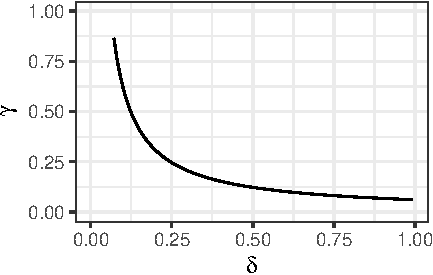
\includegraphics{sensitivity_analysis_files/figure-beamer/unnamed-chunk-9-1} \end{center}

\normalsize

\begin{itemize}
\tightlist
\item
  What does this curve represent?
\end{itemize}

\end{frame}

\begin{frame}[fragile]{}

\begin{itemize}
\tightlist
\item
  How are the covariates related to the treatment?
\end{itemize}

\small

\begin{Shaded}
\begin{Highlighting}[]
\CommentTok{# Estimate the relationship between covariates (U) and treatment (D)}
\NormalTok{mod_delta <-}\StringTok{ }\KeywordTok{lm}\NormalTok{(treat }\OperatorTok{~}\StringTok{ }\NormalTok{age }\OperatorTok{+}\StringTok{ }\NormalTok{educ }\OperatorTok{+}\StringTok{ }\NormalTok{married }\OperatorTok{+}\StringTok{ }\NormalTok{black }\OperatorTok{+}\StringTok{ }\NormalTok{re75, }
           \DataTypeTok{data =}\NormalTok{ lalonde)}
\end{Highlighting}
\end{Shaded}

\normalsize

\tiny

\begin{table}[!htbp] \centering 
  \caption{OLS delta} 
  \label{} 
\begin{tabular}{@{\extracolsep{5pt}}lc} 
\\[-1.8ex]\hline \\[-1.8ex] 
\\[-1.8ex] & treat \\ 
\hline \\[-1.8ex] 
 age & 0.003 \\ 
  & (0.003) \\ 
  educ & 0.018 \\ 
  & (0.014) \\ 
  married & 0.030 \\ 
  & (0.068) \\ 
  black & 0.021 \\ 
  & (0.063) \\ 
  re75 & 0.00001 \\ 
  & (0.00001) \\ 
  Constant & 0.123 \\ 
  & (0.164) \\ 
 N & 445 \\ 
R$^{2}$ & 0.010 \\ 
\hline \\[-1.8ex] 
\end{tabular} 
\end{table}

\normalsize

\end{frame}

\begin{frame}[fragile]{}

\begin{itemize}
\tightlist
\item
  How do they relate to the outcome? \small
\end{itemize}

\begin{Shaded}
\begin{Highlighting}[]
\CommentTok{# Estimate relationship between covariates (U) and outcome (Y)}
\NormalTok{mod_gamma <-}\StringTok{ }\KeywordTok{lm}\NormalTok{(re78 }\OperatorTok{~}\StringTok{ }\NormalTok{age }\OperatorTok{+}\StringTok{ }\NormalTok{educ }\OperatorTok{+}\StringTok{ }\NormalTok{married }\OperatorTok{+}\StringTok{ }\NormalTok{black }\OperatorTok{+}\StringTok{ }\NormalTok{re75, }
           \DataTypeTok{data =}\NormalTok{ lalonde)}
\end{Highlighting}
\end{Shaded}

\normalsize

\tiny

\begin{table}[!htbp] \centering 
  \caption{OLS gamma} 
  \label{} 
\begin{tabular}{@{\extracolsep{5pt}}lc} 
\\[-1.8ex]\hline \\[-1.8ex] 
\\[-1.8ex] & re78 \\ 
\hline \\[-1.8ex] 
 age & 58.494 \\ 
  & (39.976) \\ 
  educ & 440.036$^{}$ \\ 
  & (165.095) \\ 
  married & $-$122.549 \\ 
  & (864.001) \\ 
  black & $-$2,161.909$^{}$ \\ 
  & (734.904) \\ 
  re75 & 0.154 \\ 
  & (0.103) \\ 
  Constant & 941.146 \\ 
  & (2,058.587) \\ 
 N & 445 \\ 
R$^{2}$ & 0.037 \\ 
\hline \\[-1.8ex] 
\end{tabular} 
\end{table}

\normalsize

\end{frame}

\begin{frame}[fragile]{}

\begin{itemize}
\item
  To compare the hypothetical degree of confounding based on the
  sensitivity parameters with the actual degree of confounding created
  by some observed covariates, we plot them against the curve.
\item
  We use the standardized coefficients here, but you can also calculate
  the raw \(\delta\) and \(\gamma\) values, or compute the partial
  R-squared.\footnote<.->{Both standardized coeffs and partial r measure
    the unique contribution of a covariate in a model.}
\end{itemize}

\small

\begin{Shaded}
\begin{Highlighting}[]
\KeywordTok{library}\NormalTok{(lm.beta)}
\CommentTok{# Extract standardized coefficients for age}
\NormalTok{delta_age <-}\StringTok{ }\KeywordTok{abs}\NormalTok{(}\KeywordTok{lm.beta}\NormalTok{(mod_delta)}\OperatorTok{$}\NormalTok{standardized.coefficients[}\DecValTok{2}\NormalTok{])}
\NormalTok{gamma_age <-}\StringTok{ }\KeywordTok{abs}\NormalTok{(}\KeywordTok{lm.beta}\NormalTok{(mod_gamma)}\OperatorTok{$}\NormalTok{standardized.coefficients[}\DecValTok{2}\NormalTok{])}
\end{Highlighting}
\end{Shaded}

\normalsize

\end{frame}

\begin{frame}{}

\begin{itemize}
\tightlist
\item
  Do this for other covariates in the model\ldots{}
\end{itemize}

\begin{center}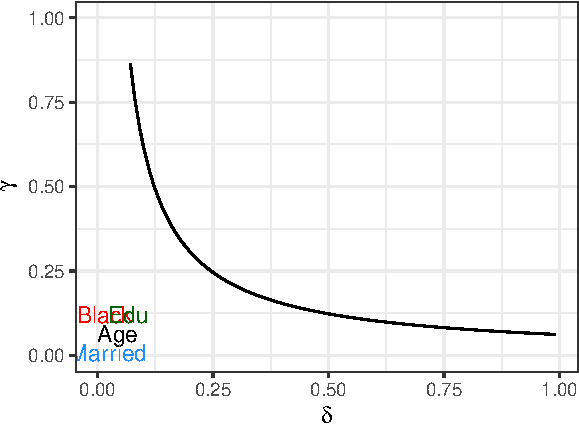
\includegraphics{sensitivity_analysis_files/figure-beamer/unnamed-chunk-16-1} \end{center}

\end{frame}

\begin{frame}{Return to Randomization Inference (Rosenbaum approach)}

\begin{itemize}
\tightlist
\item
  Components of RI:

  \begin{itemize}
  \tightlist
  \item
    Null hypothesis (i.e.~no treatment effect)
  \item
    Test-statistic (i.e.~Wilcoxon Signed Rank Test)
  \item
    Number of permutations: \emph{nCr}
  \item
    p-value is ratio of number of times we observe the test-statistic or
    greater to number of permutations
  \end{itemize}
\item
  Overview of Rosenbaumian SA:
\end{itemize}

\begin{enumerate}
\def\labelenumi{\arabic{enumi}.}
\tightlist
\item
  Set \(\Gamma\) (the sensitivity parameter).\footnote<.->{\(\Gamma = 1\)is
    the case where there is no bias from confounding.
    \color{red}{$\Gamma = 2$?}}
\item
  Compute probability of treatment (\(\pi(X_i)\)) for \(\Gamma\) bounds
  (see lecture slides).
\item
  Conduct RI under the null of
  \(min\{\pi(X_i)\} = max\{\pi(X_i)\} = 0.5\).
\item
  Repeat for different values of \(\Gamma\).
\end{enumerate}

\end{frame}

\begin{frame}{Wilcoxon Signed Rank Statistic}

\begin{itemize}
\tightlist
\item
  Wilcoxon \color{red}{Signed} \color{blue}{Rank}
  \color{violet}{Statistic}
\end{itemize}

\small

\begin{center}
 \begin{tabular}{||c c c c c c||} 
 \hline
 Match A &  7 &  5 & 3 & 4 & 1  \\ 
 \hline
 Match B & 2 & 4 &  3 & 1 & 2  \\
 \hline\hline
 Abs Diff & 5 & 1 & 0 & 3 & 1  \\  
 \hline
 \color{red}{Sign} & + & + & NA & + & -  \\ 
 \hline
 \color{blue}{Rank} & 4.0 & 1.5 & NA & 3.0 & 1.5  \\ 
 \hline
\end{tabular}
\end{center}

\normalsize

\begin{itemize}
\tightlist
\item
  \color{violet}{$W = \sum^{N}_i\{S_i\times R_i\}$}
  \color{black}{where $N$ is the number of pairs where the difference $\neq 0$, $S$ is the sign of the matched pairs ($X_{i} - X_{j}$), and $R$ denotes the rank.}
\end{itemize}

\end{frame}

\begin{frame}[fragile]{}

\begin{itemize}
\tightlist
\item
  \color{red}{Why is it necessary to match first?}
\end{itemize}

\small

\begin{Shaded}
\begin{Highlighting}[]
\NormalTok{covars <-}\StringTok{ }\KeywordTok{c}\NormalTok{(}\StringTok{"age"}\NormalTok{, }\StringTok{"educ"}\NormalTok{, }\StringTok{"black"}\NormalTok{, }\StringTok{"re75"}\NormalTok{)}
\NormalTok{matched_dat <-}\StringTok{ }\KeywordTok{Match}\NormalTok{(}\DataTypeTok{Y =}\NormalTok{ lalonde}\OperatorTok{$}\NormalTok{re78, }\DataTypeTok{Tr =}\NormalTok{ lalonde}\OperatorTok{$}\NormalTok{treat, }
                     \DataTypeTok{X =}\NormalTok{ lalonde[,covars], }\DataTypeTok{Weight =} \DecValTok{2}\NormalTok{)}

\KeywordTok{summary}\NormalTok{(matched_dat)}
\end{Highlighting}
\end{Shaded}

\begin{verbatim}
## 
## Estimate...  1913.8 
## AI SE......  821.46 
## T-stat.....  2.3297 
## p.val......  0.019819 
## 
## Original number of observations..............  445 
## Original number of treated obs...............  185 
## Matched number of observations...............  185 
## Matched number of observations  (unweighted).  301
\end{verbatim}

\normalsize

\end{frame}

\begin{frame}[fragile]{\texttt{rbounds} package}

\begin{itemize}
\tightlist
\item
  \texttt{psens} gives Rosenbaum's bounds for the p-values from a
  Wilcoxon signed rank test.
\end{itemize}

\small

\begin{Shaded}
\begin{Highlighting}[]
\KeywordTok{library}\NormalTok{(rbounds)}
\NormalTok{rosenbaum <-}\StringTok{ }\KeywordTok{psens}\NormalTok{(matched_dat, }\DataTypeTok{Gamma =} \FloatTok{1.5}\NormalTok{, }\DataTypeTok{GammaInc =} \FloatTok{0.1}\NormalTok{)}
\end{Highlighting}
\end{Shaded}

\normalsize

\begin{table}[ht]
\centering
\scalebox{0.75}{
\begin{tabular}{rrrr}
  \hline
 & Gamma & Lower bound & Upper bound \\ 
  \hline
1 & 1.000 & 0.002 & 0.002 \\ 
  2 & 1.100 & 0.000 & 0.014 \\ 
  3 & 1.200 & 0.000 & 0.057 \\ 
  4 & 1.300 & 0.000 & 0.154 \\ 
  5 & 1.400 & 0.000 & 0.306 \\ 
  6 & 1.500 & 0.000 & 0.488 \\ 
   \hline
\end{tabular}
}
\caption{Rosenbaum p-values} 
\end{table}

\begin{itemize}
\tightlist
\item
  Still need to benchmark these hypothetical values against your data by
  calculating the odds ratios!
\end{itemize}

\end{frame}

\section{Additional Notes}\label{additional-notes}

\begin{frame}{Plot twist!}

\begin{itemize}
\item
  \(\Gamma\) can be decomposed into the strength of the relationship
  between confounder and outcome (\(\Delta\)) and strength of the
  relationship between the confounder and treatment (\(\Lambda\)) as
  \[\Gamma = \frac{\Delta\Lambda + 1}{\Delta + \Lambda}\]
\item
  Details in Rosenbaum and Silber (2009).
\end{itemize}

\end{frame}

\end{document}
